\documentclass[twocolumn, prl, nobalancelastpage, aps, citeautoscript, longbibliography, 10pt]{revtex4-1}
\usepackage{geometry, graphics, bm, tikz, amsmath}
\renewcommand{\baselinestretch}{0.95}


\begin{document}

\title{Runge-Kutta Methods: Simulating Orbital Trajectories}
\author{S. A. Hopkins}
\affiliation{Level 5 Labratory, School of Physics, University of Bristol}
\date{\today}

\maketitle
\section{Introduction}
The scenario presented in the notes involved a single moving body moving within a fixed gravitational potential. This involved imploying the fourth-order Runge-Kutta
method in order to solve the following differential equation;

\begin{equation}
    m\ddot{\boldsymbol{r}} = -\frac{mMG}{|\boldsymbol{r}|^2}\hat{\boldsymbol{r}} = - \frac{mMG}{|\boldsymbol{r}|^3}\boldsymbol{r} 
\end{equation}
The differential describes the motion of a single body, where $M$ is the mass of the planet, $m$ is the mass of the rocket, $\boldsymbol{r}$ is the distance from the centre of mass
of the planet to the rocket, and $G$ is the gravitational constant. In order to solve this ordinary differential equation, we solve for $\boldsymbol{r}$, using an iterative method 
in numerical analysis, called the Runge-Kutta method. 
\subsection{Runge-Kutta Method}
The Runge-Kutta approach is an iterative and explicit method, used to provide approximate solutions to ordinary differential equations through temporal discretisation, in which 
we require an integral of every term for each time-step, $h$. The most well-known of these methods is the fourth order Runge-Kutta method (RK4). The RK4 method evaluates the slope
of a given function, at four points in a given interval, provided the initial conditions are known. We can summarise this as;
\begin{align}
k_1 &= f(x_n, y_n), \\
k_2 &= f(x_n + \frac{h}{2}, y_n + \frac{hk_1}{2}), \\
k_3 &= f(x_n + \frac{h}{2}, y_n + \frac{hk_1}{2}), \\
k_4 &= f(x_n + h, y_n + hk_3)
\end{align}
Here, $x$ and $y$ are the positional coordinates of the satellite and components of $\bm{r}$, $h$ is the time-step, $k_1$ is the slope at the beginning of the interval, $k_2$
is the slope at the midpoint of the interval, calculated using $k_1$, $k_3$ is the slope at the midpoint of the interval, calculated using $k_2$, $k_3$ is the slope at the end of the 
interval. This is the summary of the method to which we can arrive at a solution, given as;
\begin{equation}
    y_{n+1} = y_n + \frac{h}{6}\left[k_1 + 2k_2 + 2k_3 + k_4\right] +\mathcal{O}(h^5)
\end{equation}
It can be seen in Eq.(6) that the local truncation error on the solution is of order $\mathcal{O}(h^5)$, while the total accumulated error is on the order of $\mathcal{O}(h^4)$, 
hence the name, 'Fourth Order Runge-Kutta'. For the scenario presented, where there are two dependent variables, we can write the solutions as;

\begin{align}
    \bm{\mathrm{x}}_{i+1}& = \bm{\mathrm{x}}_i + \frac{h}{6}\left[k_1 + 2k_2 + 2k_3 + k_4\right],\\
    t_{i+1}& = t_i + h,
\end{align}
where $\bm{\mathrm{x}}$ is the vector that contains all the dependent variables. See the appendix for the full set of equations that were used in the exercise. 

\section{Results}
\begin{figure}[h!]
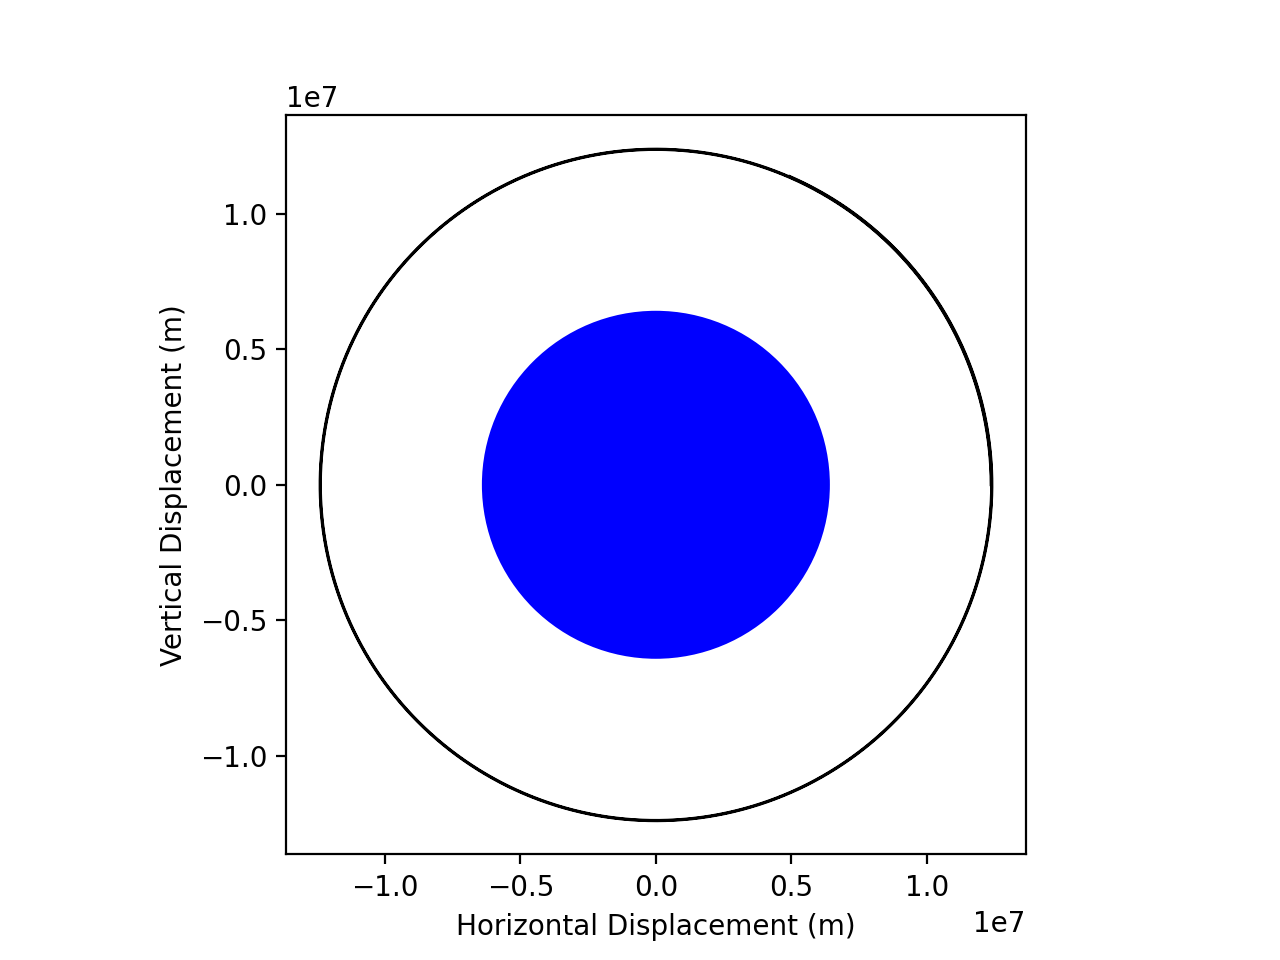
\includegraphics[width = 0.96\linewidth]{CircularOrbit2d.png}
\caption{Orbital trajectory of a satellite in circular orbit with an initial veloctity of $8529.93$m/s and initial height of $12.37\times10^3$km. The blue object represents
earth, while the black line represents the path of the satellite. The simulation was ran for $30000$s with a time-step of $1s$ }
\label{CircularOrbit}
\end{figure}
In the simulation, 4 different types of orbits were plotted and investigated. The first two orbits, involved a moving body orbiting a single massive body, while the last two, involved
a body orbiting an Earth-Moon system. For the single massive body conditions, two trajectories were plotted. The first was a circular orbit and the second was an elliptical
orbit. The circular orbit was plotted for $30000$s with an initial velocity of $8529.93$m/s and an initial height of $12.37\times10^3$km. As shown in Figure \ref{CircularOrbitEnergy}, 
the energy remained constant for the whole trajectory, implying that the orbit was stable and stayed along the same height it was set at initially. The initial velocity 
was calculated using;
\begin{equation}
    v = \sqrt{\frac{G M_E}{x_0}}
\end{equation}
where $x_0$ is the initial height of the satellite, and $M_E$ is the mass of the Earth.


\begin{figure}[h!]
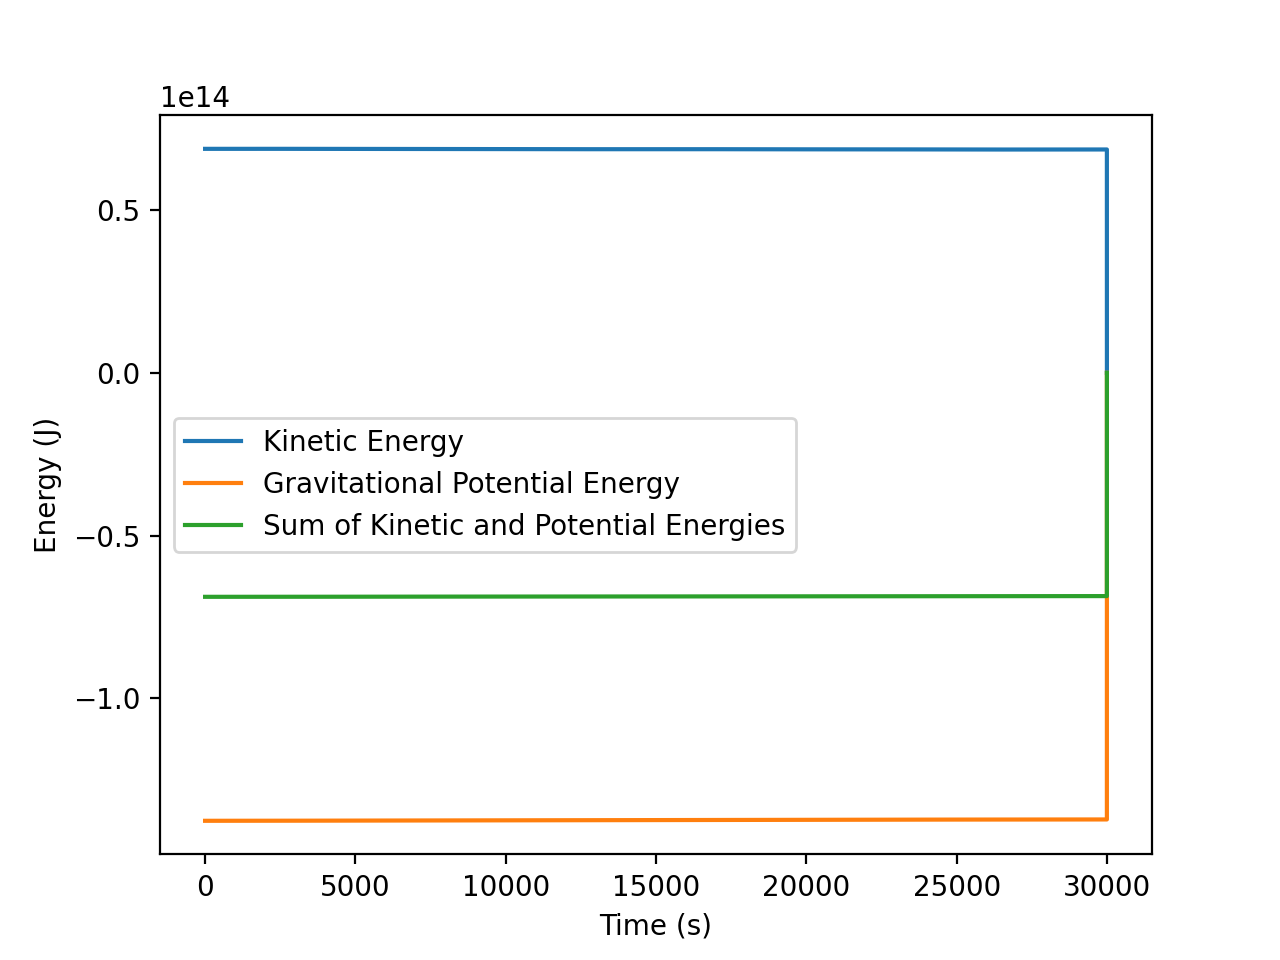
\includegraphics[width = 0.96\linewidth]{CircularOrbitEnergy.png}
\caption{Energy plot for the orbital trajectory plotted in Figure \ref{CircularOrbit}. Kinetic energy for the whole flight is shown by the blue line, gravitational energy 
is represented by the orange line, and the sum of the two energies is shown by the green line.}
\label{CircularOrbitEnergy}

\end{figure}
The second orbit was an elliptical orbit that ran for $293527$s, with initial velocity of $7600$m/s and initial height $12.37\times10^3$km. Again, a time-step of 1 was used. Figure \ref{EllipticalOrbitEnergy} shows the 
energy over time for the flight, and it can be seen that the energy is conserved for the entire flight with 3 major peaks. These peaks occur at the point 
when the satellite is closest to the earth. This graph also shows that the sum of the kinetic and potential energies is constant, 
implying that energy is conserved for the flight. The initial velocity for the flight was determined by starting at $8000$m/s and lowering
the value until a desired orbit is achieved. 

\begin{figure}[h]
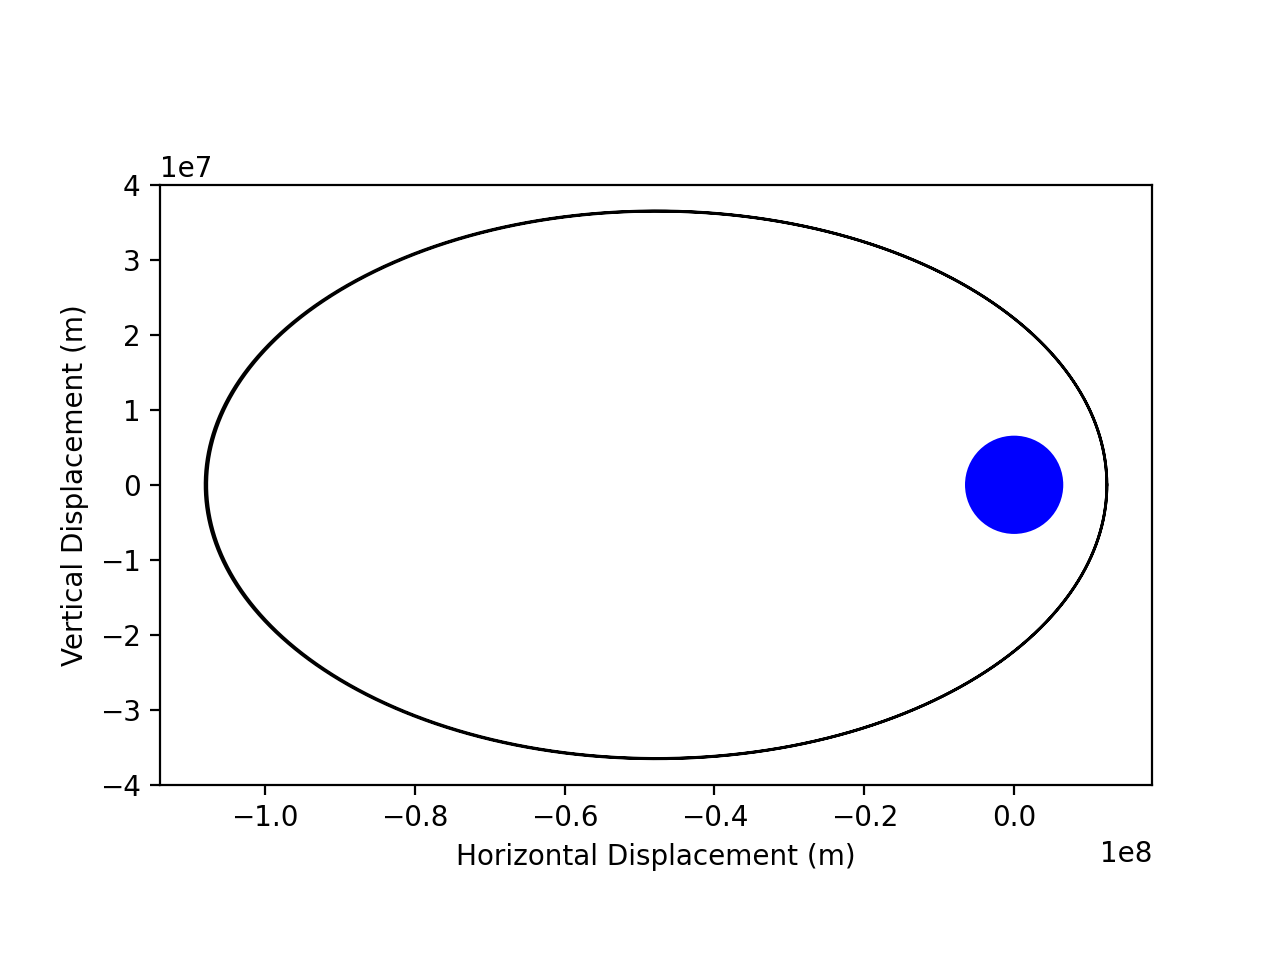
\includegraphics[width = 0.96\linewidth]{EllipticalOrbit2d.png}
\caption{Orbital trajectory of a satellite in an elliptical orbit with an initial velocity of $7600$m/s and initial height of $12.37\times10^3$km. The blue object represents Earth
and the black line represents the satellites trajectory. The simulation was ran for $293527$s, with a time-step of $1$s}
\label{EllipticalOrbit}
\end{figure}
\begin{figure}[h!]
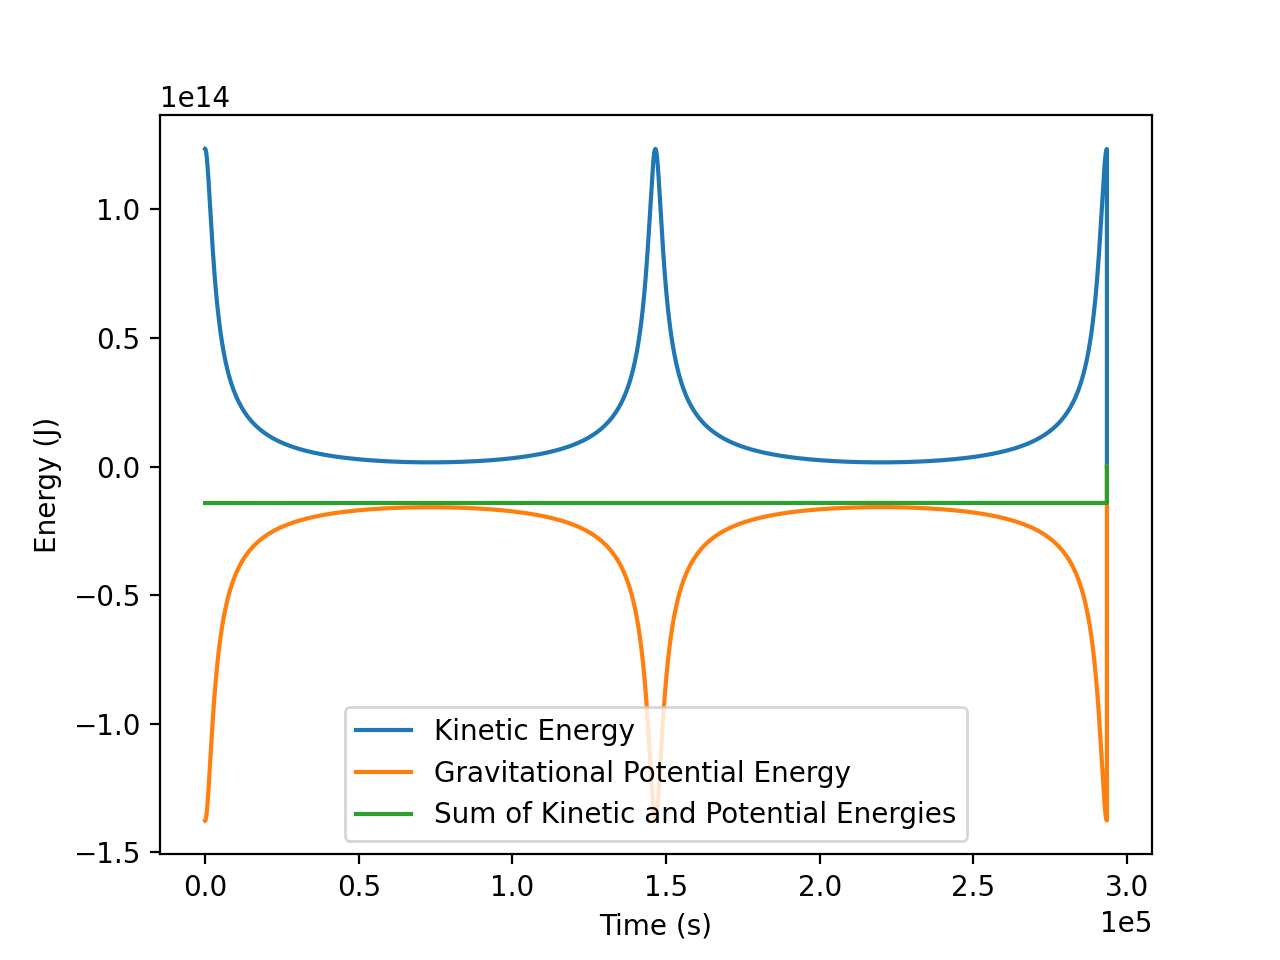
\includegraphics[width = 0.96\linewidth]{EllipticalEnergy.png}
\caption{Energy plot for the orbital trajectory plotted in Figure \ref{EllipticalOrbit}. Kinetic energy for the whole flight is shown by the blue line, gravitational energy 
is represented by the orange line, and the sum of the two energies is shown by the green line.}
\label{EllipticalOrbitEnergy}
\end{figure}

\subsection{Earth-Moon Orbit}
The goal of this section was to launch a rocket from low earth orbit, such that it passes over the Moon's surface to take photographs, 'slingshots'
around the moon, and then passes close to earth once more to send back the information by radio. There is only enough fuel for one rocket burn.
In order to simulate this, the derivatives from the first section had to be changed in order to account for the separation of the earth and the moon,
aswell as the gravitational effect due to the moon. Two different types of stable orbits were able to be plotted. The first was the elliptical orbit that 
went around the moon fully, and the second was the figure-of-eight orbit. Both orbits required tremendous trial and error to find 
the initial condtions, as the simulation took a long time to run and was very susceptible to the initial velocity. In order to find the initial velocity 
for both orbits, i employed the same method as for the elliptical orbit to achieve the plots shown in figures \ref{SlingshotOrbit} and \ref{Figureof8Orbit}.



\begin{figure}[p!]
    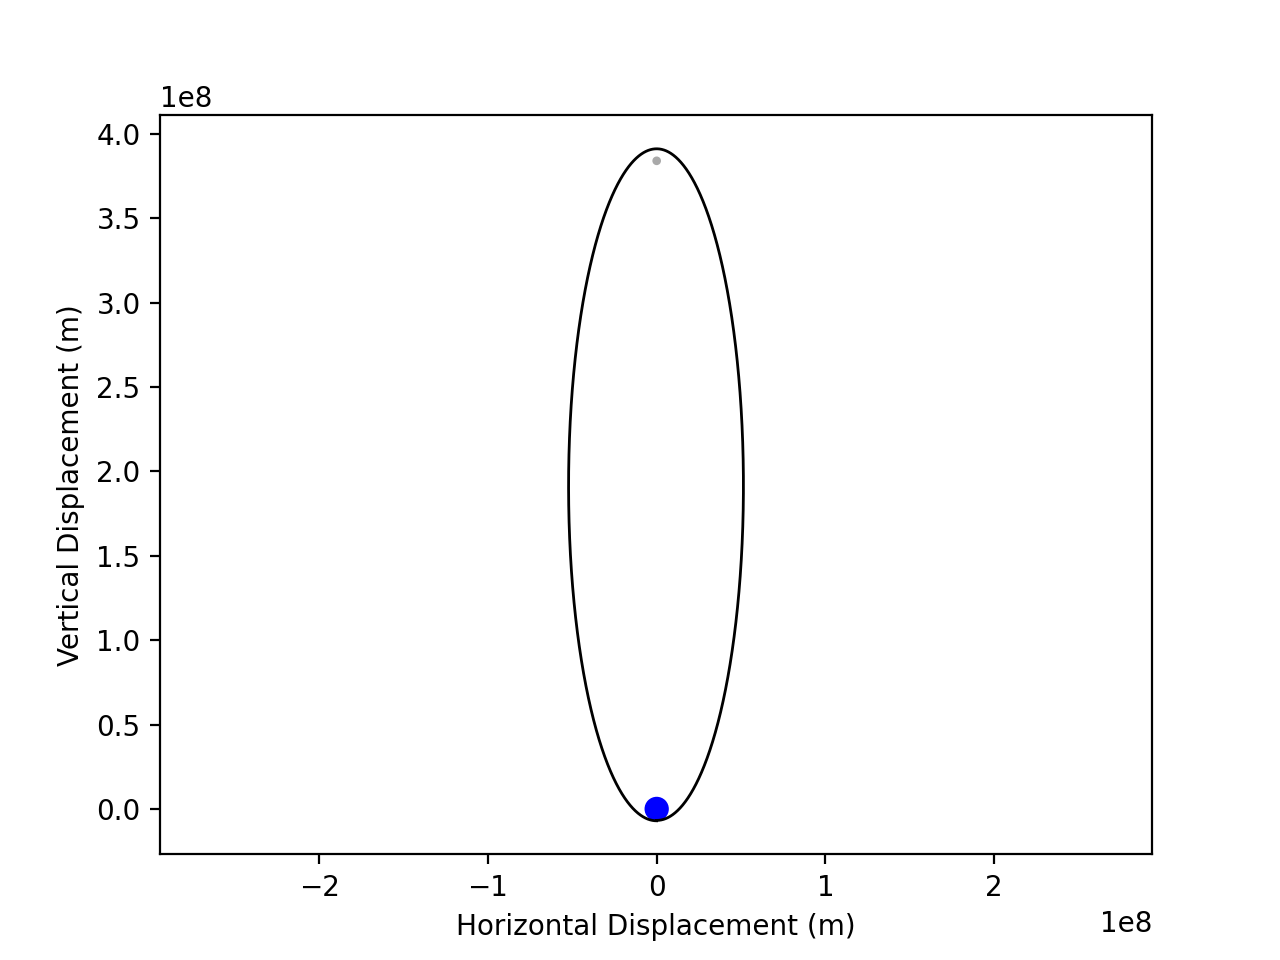
\includegraphics[width = 0.96\linewidth]{Earth-MoonOrbit.png}
    \caption{Orbital trajectory of the satellite for the Earth-Moon system. The initial velocity was $10729.6$m/s and the initial height was set it $6800\times10^3$km. The grey object represents
    the moon and the blue object represents the earth. The simulation ran for $647075$s with a time-step of $1$s.}
    \label{SlingshotOrbit}
\end{figure}
\begin{figure}[p!]
    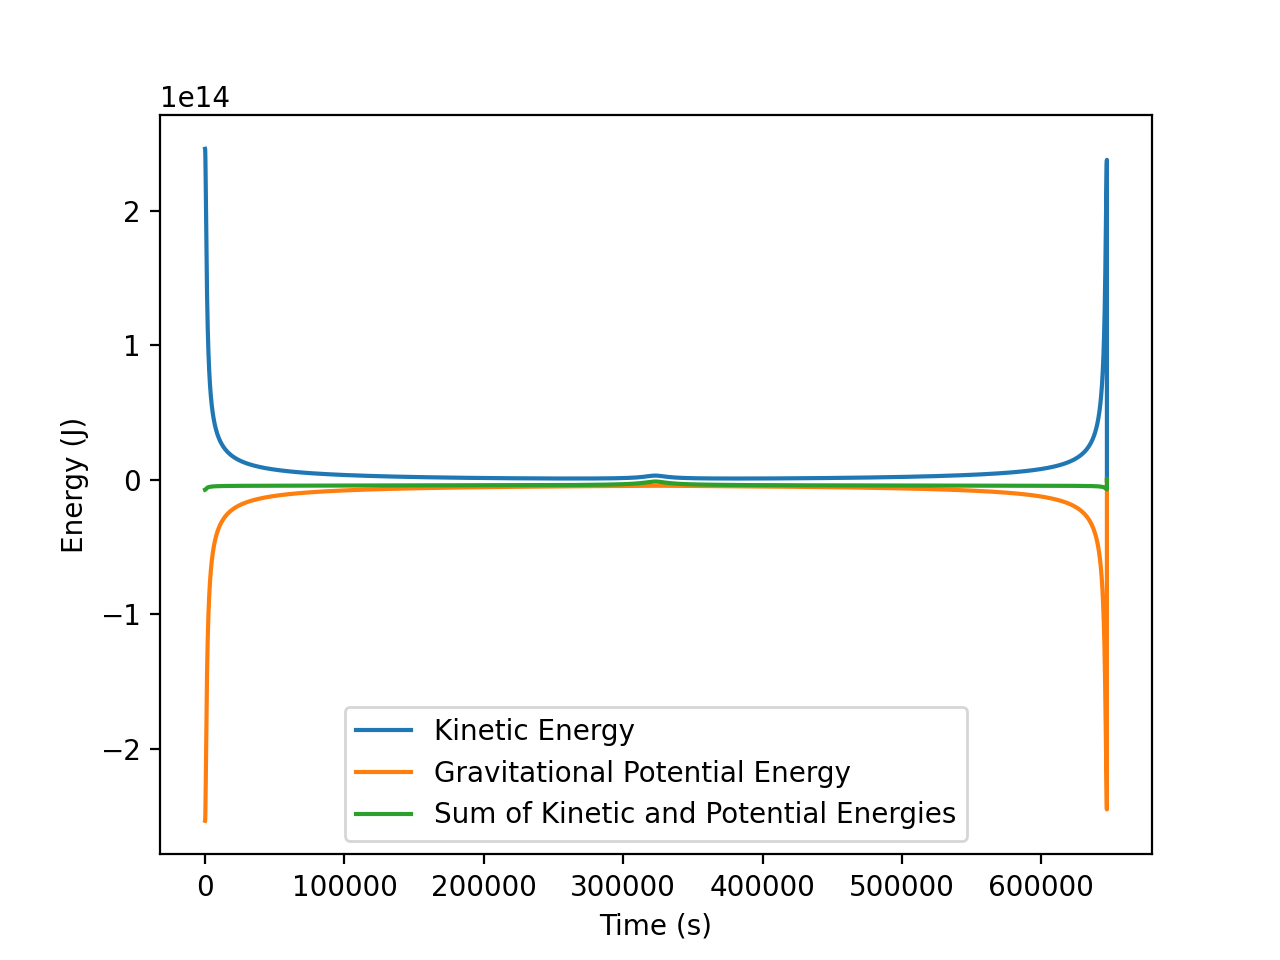
\includegraphics[width = 0.96\linewidth]{Earth-MoonEnergy.png}
    \caption{Energy plot for the trajectory shown in figure \ref{SlingshotOrbit}. Kinetic energy for the whole flight is shown by the blue line, gravitational energy 
    is represented by the orange line, and the sum of the two energies is shown by the green line. }
    \label{SlingshotEnergy}
\end{figure}
\begin{figure}[p!]
    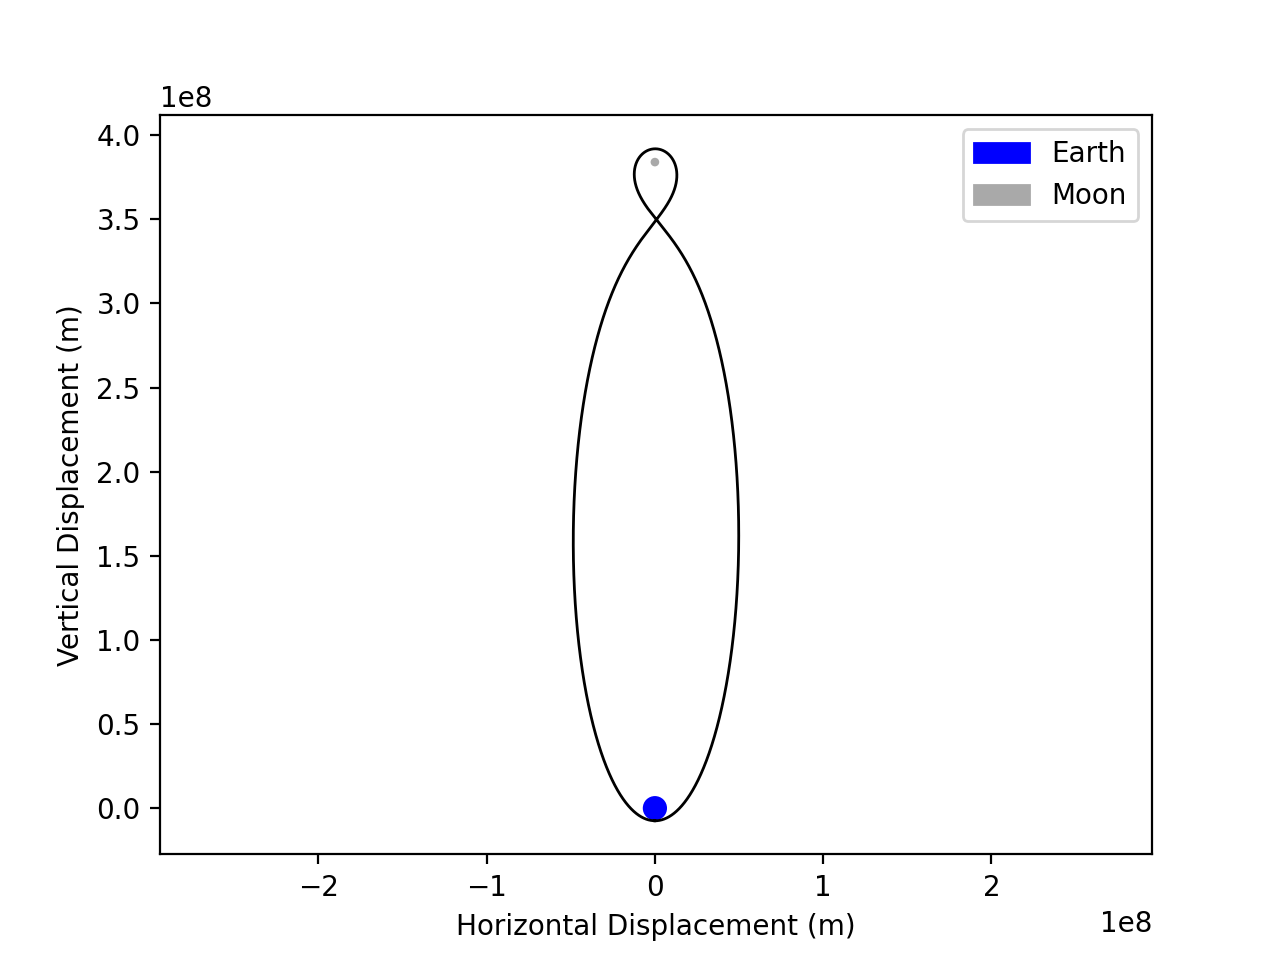
\includegraphics[width = 0.96\linewidth]{Figureo8Orbit.png}
    \caption{Orbital trajectory of the satellite for the Earth-Moon system for the figure-of-eight orbit. The initial velocity was $10191$m/s and the initial height was set it $7500\times10^3$km. The grey object represents
    the moon and the blue object represents the earth. The simulation ran for $828671$s with a time-step of $1$s.}
    \label{Figureof8Orbit}
\end{figure}
\begin{figure}[p!]
    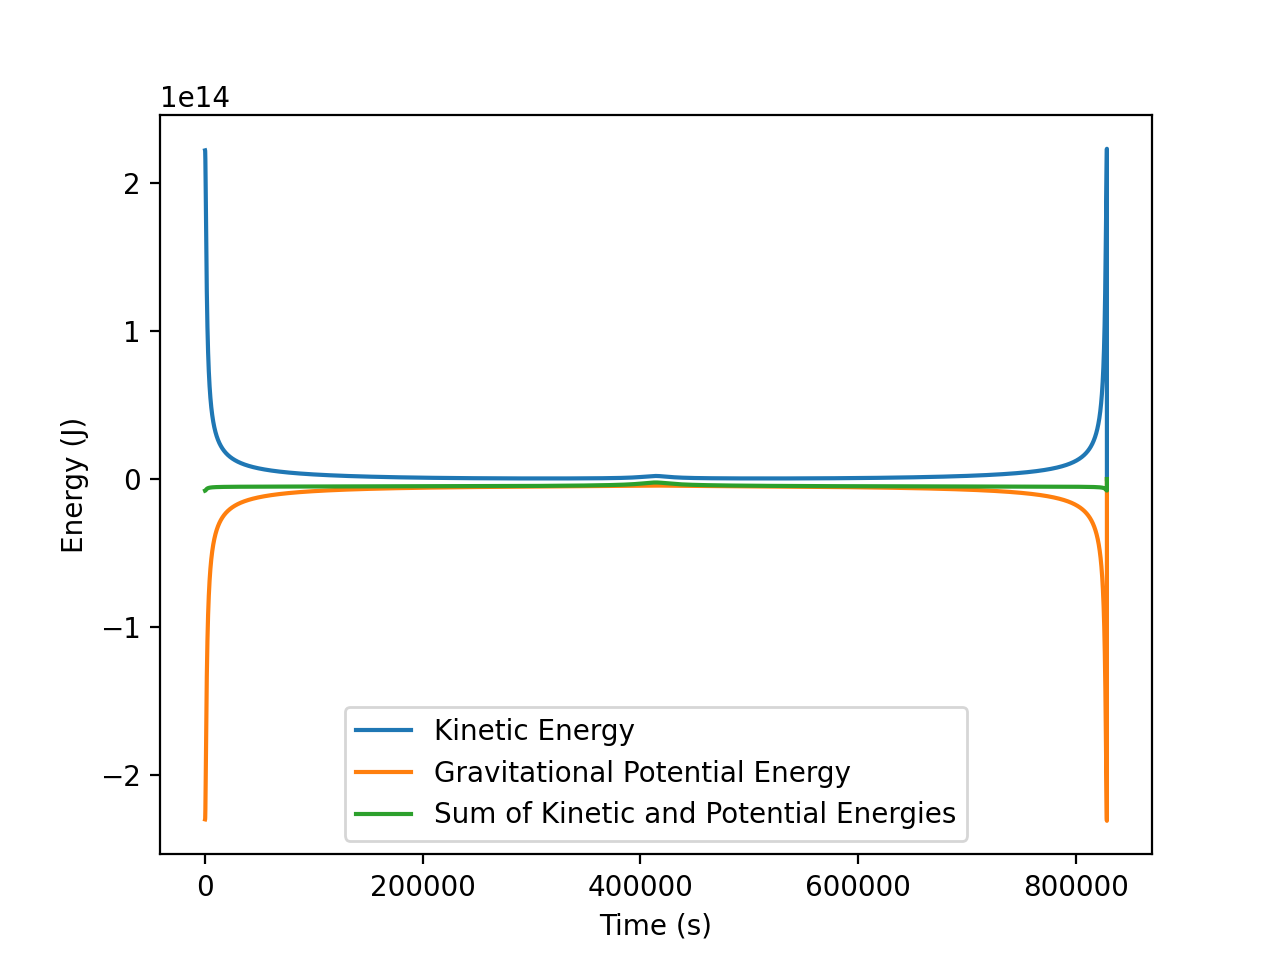
\includegraphics[width = 0.96\linewidth]{Figureo8Energy.png}
    \caption{Energy plot for the trajectory shown in figure \ref{Figureof8Orbit}. Kinetic energy for the whole flight is shown by the blue line, gravitational energy 
    is represented by the orange line, and the sum of the two energies is shown by the green line. }
    \label{SlingshotEnergy}
\end{figure}







\section{Improvements}
One of the main improvements to the code, would be to numerically specify the errors in the solutions provided by the RK4 method. This could have been done by calculating the difference between 
the initial and final energy, as they should be the same if energy is conserved. One of the main problems that arose when trying to implement this, was that
the energy calculated for the last time slot in the time-array turned out to be 0. This is due to how the code was written, and I could not
think of a way to specify this last value to be non-zero. This can be clearly seen in the graphs, where all three lines jump from their respective values
to 0 right at the end of the simulation. Another possible improvement, would be to animate the trajectory of the satellite, as this is a perfect
use-case for animation with python. This is a little outside my area of knowledge however, hence it not being implemented. One final improvement
could be to use a more object oriented programming style, making the code much more easier to read, as i tried to implement this at the start, but time restrictions prevented me from 
implementing this further. 
\end{document}